\documentclass[8pt]{extarticle}

\usepackage[utf8]{inputenc}
\usepackage[russian]{babel}
\usepackage{amsmath}
\usepackage{graphicx}
\usepackage[colorinlistoftodos]{todonotes}

\usepackage{listings}
\lstset{language=Haskell}

\title{Шаблон проектирования View в языках с зависимыми типами}

\author{Марат Хабибуллин}

\date{\today}

\begin{document}
\maketitle

\begin{figure}[!htbp]
\centering
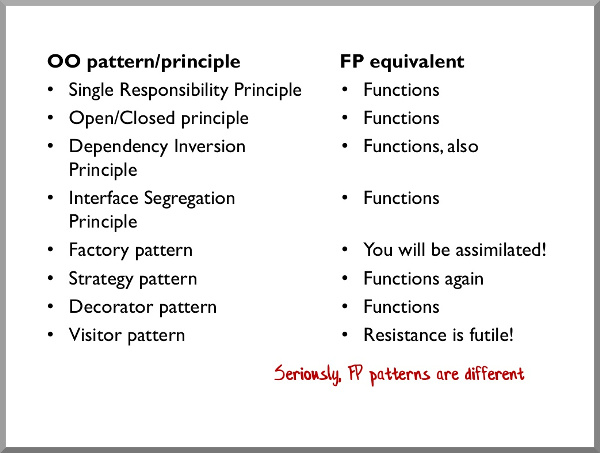
\includegraphics[width=1\textwidth]{fp_patterns.jpg}
\end{figure}

\section{Вступление}

Шаблоны проектирования! Впервые я узнал о них на курсе Software Design, когда учился в магистратуре Академического университета. Мы писали различные программы на Java с использованием шаблонов. С тех пор это словосочетание ассоциируется у меня с чем-то таким ООПшным. Однако, разбираясь с языком Agda, я наткнулся на статью The Power Of Pi, которая рассказывает про шаблоны проектирования в языках с зависимыми типами!\\
В этом посте я хочу рассказать об одном из этих шаблонов, который называется View. С его помощью можно реализовывать пользовательские правила pattern matching'a. Если вам интересно, что это за шаблон, что такое пользовательский pattern matching, каковы особенности pattern matching'а в языках с зависимыми типами, и вы знакомы с каким-нибудь функциональным языком программирования со статической типизацией (Haskell, Scala, Ocaml, F\#) -- добро пожаловать под кат!


\section{Views и пользовательский pattern matching}

Для начала разберёмся, что такое пользовательский pattern matching. Пусть мы работаем с каким-нибудь списком xs и выполняем на нём pattern matching:
\begin{lstlisting}
match xs with 
	[] -> ...
	(y : ys) -> ...
\end{lstlisting}
Здесь мы смотрим на xs либо как на пустой список, либо как на список, состоящий из головного элемента и приписанный к нему списка. Но что если мы хотим посмотреть на xs, скажем, как на список, состоящий из конкатенации некоторых двух списков ys и zs? Что-то вроде
\begin{lstlisting}
match xs with
	[] -> ...
	(ys ++ zs) -> ...
\end{lstlisting}
Иными словами, нам хочется влиять на то, как именно будет представляться структура данных в результате pattern matching'a. Это мы и будем называть пользовательским pattern matching'ом.\\
\\
По ходу статьи, нашей целью будет реализация пользовательского pattern matching'а для следующей ситуации. Пусть мы работаем с битовыми векторами фиксированной длины. При этом, у нас есть возможность указывать длину вектора прямо в типе. К примеру, запись bits : [32] означает, что bits -- это 32-битный вектор. Мы, в процессе pattern matching'а, хотим иметь возможность различными способами разбивать вектор на равные части, к примеру, так:
\begin{lstlisting}
swapAB : [32] -> [32]
swapAB [a b c d] = [b a c d]
\end{lstlisting}
Эта функция принимает на вход 32-битный вектор, разбивает его на 4 части, каждая из которых является 8-битным вектором, и меняет первые два 8-битных слова местами. Она, с тем же успехом, могла разбить его и на 2 части, каждая по 16-бит. Такой функционал может быть полезен при написании криптографического ПО. К примеру, нечто подобное лежит в основе языка Cryptol, который заточен под написание криптографических алгоритмов. Посмотрим, как реализовать такое на Agda.\\
\\
Общая схема реализации пользовательского pattern matching'а будет такая:
\begin{enumerate}
\item Реализовать шаблон View для исходного типа данных: 

\begin{enumerate}
\item Определить тип данных View, конструкторы которого представляют значения исходного типа в нужном нам виде.
\item Написать функцию view, которая по значению исходного типа данных строит значение типа View.
\end{enumerate}

\item Использовать pattern matching на результах вызова функции view
\end{enumerate}
Перед тем как разбираться с этими пунктами, определим некоторые базовые типы данных.


\subsection{Натуральные числа и вектор в Agda}

Натуральные числа определяются рекурсивно:
\begin{lstlisting}
data Nat : Set where
  Zero : Nat
  Suc  : Nat -> Nat
\end{lstlisting}
При определении типа Nat, мы указываем его тип! Так же как число 3 имеет тип Nat, сам по себе тип Nat имеет тип Set. Set -- это встроенный тип Agda. Однако, понимание, зачем это нужно, нам не пригодится, и можно просто считать, что все типы имеют тип Set, хотя это не правда.\\
У типа Nat два конструктора: Zero, у которого нет аргументов, и Suc -- конструктор с одним аргументом. Число 3, таким образом, выглядит как (Suc (Suc (Suc zero))), то есть что-то вроде (1 + (1 + (1 + 0))). Однако, в Agda есть встроенные литералы, поэтому вместо длинной цепочки Suc можно просто писать 3.\\
\\
Вектор -- это список фиксированной длины, определяется так:
\begin{lstlisting}
data Vec (A : Set) : Nat -> Set where
	[] : Vec A Zero
	_::_ : {n : Nat} -> A -> Vec A n -> Vec A (Suc n)
\end{lstlisting}
Тип Vec, в отличие от Nat, имеет 2 параметра: тип A и значение типа Nat. Благодаря тому, что второй параметр Vec -- это значение, а не тип, Vec является зависимым типом. Тот факт, что параметры отделены друг от друга двоеточием, а не, скажем, символом '->' -- не совпадение. На самом деле, то, что записано после двоеточия -- это так называемые индексы, а не параметры. Однако, для нас это отличие не будет играть особого значения и мы будем всё называть параметрами.\\
Первый конструктор строит пустой вектор. В Agda в качестве имён можно использовать разные последовательности символов, поэтому мы можем назвать конструктор [].\\
Второй конструктор принимает 3 аргумента -- размер вектора n, элемент вектора типа A, вектор размера n, и возвращает вектор размера (n + 1). Заметим, что для первого аргумента, равно как и для первого параметра самого типа Vec, мы указали не просто тип, но и имя -- n : Nat. Это нужно, потому что мы ссылкаемся на это значение при объявлении третьего аргумента и возвращаемого значения. Кроме того, первый аргумент взят в фигурные скобки. Так в Agda обзначаются неявные аргументы. Дело в том, что значение n можно однозначно восстановить из третьего аргумента конструктора. Действительно, когда мы передаём вектор, мы знаем его размер, он указан в типе. Поэтому, на самом деле, первый аргумент мы можем не передавать -- Agda сама догадается, какой он должен быть. Таким образом, вызов конструктора \_::\_ выглядит либо как '\_::\_ \{n\} a someVec', либо как '\_::\_ a someVec'. Но и это ещё не всё! Символы подчёркивания в имени конструктора, на самом деле, говрят о том, что он является инфиксным. Два явных аргумента можно писать не после имени конструктора, а вместо подчёркиваний, разделяя всё это пробелами. В итоге, вот пример создания вектора:
\begin{lstlisting}
v1 : Vec Nat 2
v1 = 1 :: (2 :: [])
\end{lstlisting}
Заметьте, что мы не можем писать так:
\begin{lstlisting}
v1 : Vec Nat 3
v1 = 1 :: (2 :: [])
\end{lstlisting}
Конструктор [] создаёт вектор длины 0, первый конструктор :: -- вектор длины 1, второй :: -- вектор длины 2. Получаем Vec Nat 2, а надо 3. Система вывода типов не даст нам компилировать такой код.\\
\\
Кроме всего прочего, нам понадобятся некоторые операции над векторами:
\begin{lstlisting}
_++_ : forall {A m n} -> Vec A m -> Vec A n -> Vec A (m + n)
take : forall {A m} -> (n : Nat) -> Vec A (n + m) -> Vec A n
drop : forall {A m} -> (n : Nat) -> Vec A (n + m) -> Vec A m
\end{lstlisting}
Это конкатенация векторов, операция 'взять первые n элементов' и 'выбросить первые n элементов', аналогичные тем, что есть для списка в Haskell. Запись вроде 'forall \{A m n\}' означает, что, помимо того, что аргументы A, m и n неявные, так мы ещё и не хотим указывать их тип и просим Agda определить его на основе явных аргументов, что опять же происходит очевидным образом.


\subsection{Тип битового вектора}

Тип битового вектора, для которого мы будем реализовывать pattern matching, будет выглядеть довольно просто:
\begin{lstlisting}
data Bit : Set where
	O : Bit
	I : Bit

Word : Nat -> Set
Word n = Vec Bit n
\end{lstlisting}
Word -- это синоним для Vec Bit, используя его мы можем объявлять 32-битный вектор как bits : Word 32.\\
Перед тем, как перейти к pattern matching'у, посмотрим на его особенности в присутствии зависимых типов.


\subsection{Особенности pattern matching в присутствии завиcимых типов}

Рассмотрим следующий тип данных: 
\begin{lstlisting}
data _==_ {A : Set} : A -> A -> Set where
	Refl : {x : A} -> x == x
\end{lstlisting}
Тип (x == y) параметризуется двумя конкретными значениями типа A и, как несложно догадаться, представляет утверждение о том, что значения x и y равны. Наличие единственного конструктора Refl гарантирует, что мы не можем создать значения типа (x == y) для разных значений x и y. К примеру:
\begin{lstlisting}
eq : (3 == 3)
eq = Refl

notEq : (3 == 4)
notEq = ?
\end{lstlisting}
В первом случае нам нужно сконструировать значение типа (3 == 3) и у нас есть конструктор, который позволяет это сделать -- Refl. Значение же типа (3 == 4) мы сконструировать не можем -- Refl не подходит по типу, а других конструкторов у типа == нет.
\\
Теперь рассмотрим такую функцию:
\begin{lstlisting}
f : (x : Nat) -> (y : Nat) -> (x == y) -> Nat
\end{lstlisting}
Как будет выглядеть pattern matching для аргументов этой функции? Очевидно, что для третьего аргумента мы напишем Refl, так как других конструкторов у типа == нет. При этом, мы автоматически узнаём, что первый и второй аргумент -- это одно и то же число! В подобных случаях, в Agda необходимо явно отметить этот факт используя так называемый dot pattern:
\begin{lstlisting}
f x .x Refl = x
\end{lstlisting}
Такая запись означает, что второй аргумент (который имеет такое же имя как первый с приписанной точкой) -- это то же самое, что сопоставилось с первым аргументом. Мы не можем написать, скажем, 'y' вместо '.x', так как не хотим терять информацию о равенстве, которую получили после сопоставления с Refl.\\
\\
Вывод отсюда такой: в языках с зависимыми типами, после pattern matching'а на каком-либо аргументе, мы можем получить дополнительную информацию о других аргументах.


\subsection{Views}

Перед тем как построить View для нашего типа Word, рассмотрим более простой пример, чтобы понять, чего мы хотим достичь.
Рассмотрим тип списка:
\begin{lstlisting}
data List (A : Set) : Set where
	[] : List A
	_::_ : A -> List A -> List A
\end{lstlisting}
Это обычный список, такой же, как в Haskell, он представляется рекурсивно, как "первый элемент и список". Мы хотим получить возможность представить тот же самый список как "список и последний элемент". Заведём для этого тип данных SnocView:
\begin{lstlisting}
data SnocView {A : Set} : List A -> Set where
	[] : SnocView []
	_:::_ : (xs : List A) -> (x : A) -> SnocView (xs ++ (x :: []))
\end{lstlisting}
Здесь используется оператор ++ -- это конкатенация списков, как в Haskell. Пример значения типа SnocView:
\begin{lstlisting}
sx : SnocView (1 :: 2 :: 3 :: [])
sx = (1 :: 2 :: []) ::: 3
\end{lstlisting}
Заметьте, что тип SnocView параметризуется списком, для которого строится представление "список и последний элемент".\\
Теперь напишем функцию snocView, которая для переданного списка строит значение типа SnocView:
\begin{lstlisting}
snocView : {A : Set} -> (xs : List A) -> SnocView xs
snocView [] = []
snocView (x :: xs)              with snocView xs
snocView (x :: .[])                | []       = [] ::: x
snocView (x :: .(ys ++ (y :: []))) | ys ::: y = (x :: ys) ::: y
\end{lstlisting}
Здесь много всего, начнём по порядку. Случай с пустым списком очевиден: пустой список даёт тривиальный SnocView. Далее, если список не пуст, мы используем конструкцию with (длинные отступы здесь только для удобства чтения). Это конструкция выполняет примерно те же задачи, что и конструкция case of в Haskell, то есть используется для выполнения pattern matching в теле функции. Образцы, с которыми мы сопоставляем рекурсивный вызов 'snocView xs', указаны справа от вертикальных чёрточек. Итак, если рекурсивный вызов дал нам тривиальный SnocView, значит список 'xs' был пуст, поэтому SnocView для 'x :: []' -- это '[] ::: x'. Во втором случае, мы получаем, что SnocView для 'xs' выглядит как 'ys ::: y', поэтому, чтобы получить SnocView для 'x :: xs' нужно добавить 'x' в голову 'ys'.\\
Непонятным осталось лишь то, что указано слева от вертикальных чёрточек. Как мы обсуждали ранее, pattern matching в присутствии зависимых типов может давать нам дополнительную информацию о других аргументах функции. В нашем примере, pattern matching на рекурсивном вызове 'snocView xs' даёт нам информацию о том, какое значение имеет список 'xs'. Именно эта информация и указывается с помощью dot patterns слева от вертикальной черты. К примеру, во втором случае, узнав, что 'snocView xs' даёт нам 'ys ::: y', мы понимаем, что список 'xs' конструируется как конкатенация 'ys' и списка из одного элемента 'y :: []'.\\
\\
Вот пример использования snocView для написания функции, которая циклически сдвигает переданный список вправо:
\begin{lstlisting}
rotateRight : {A : Set} -> List A -> List A
rotateRight xs with snocView xs
rotateRight ._ | [] = []
rotateRight ._ | ys ::: y = y :: ys
\end{lstlisting}
Здесь мы использовали символы подчёркивания. Так можно делать, когда нас не интересует значение, которое должно быть на месте подчёркиваний. Выглядит довольно кратко и красиво! Этот пример, по сути, и показывает, как реализовывть пользовательский pattern matching в языках с зависимыми типами. Посмотрим теперь, как провернуть тоже самое для типа Word!


\subsection{SplitView для Word}

Как и в предыдущем примере, нам необходимы 2 вещи: специальный тип данных SplitView и функция splitView, которая будет строить значение SplitView для заданного значения типа Word.\\
Для начала, нам понадобятся 2 дополнительные функции для работы с типом Vec:
\begin{lstlisting}
split : forall {A} -> (n : Nat) -> (m : Nat) -> Vec A (m * n) -> Vec (Vec A n) m
split n Zero [] = []
split n (Suc k) xs = (take n xs) :: (split n k (drop n xs))

concat : forall {A n m } -> Vec (Vec A n) m -> Vec A (m * n)
concat [] = []
concat (xs :: xss) = xs ++ concat xss
\end{lstlisting}
Тип SplitView будет выглядеть так:
\begin{lstlisting}
data SplitView {A : Set} : {n : Nat} -> (m : Nat) -> Vec A (m * n) -> Set where
	[_] : forall {m n} -> (xss : Vec (Vec A n) m) -> SplitView m (concat xss)
\end{lstlisting}
Этот тип параметризуется числом m и вектором. m показывает, на сколько частей мы хотим разбить вектор. Именно поэтому длина вектора кратна m. Единственный конструктор позволит нам записывать значения данного типа так:
\begin{lstlisting}
[ a :: b :: c :: d :: [] ]
\end{lstlisting}
где a, b, c и d -- векторы длины n.\\
На очереди функция splitView:
\begin{lstlisting}
splitView : {A : Set} -> (n : Nat) -> (m : Nat) -> (xs : Vec A (m * n)) -> SplitView m xs
\end{lstlisting}
Чтобы её реализовать, нужно разбить переданный вектор на m частей, каждая длины n, и передать в конструктор [\_]:
\begin{lstlisting}
splitView n m xs = [ split n m xs ]
\end{lstlisting}
Однако, такое определение не принимается компилятором. Дело в том, что конструктор [\_] возвращает значение типа SplitView m (concat xss). В нашем случае, xss -- это 'split n m xs', так что выражение '[ split n m xs ]' имеет тип 'SplitView m (concat (split n m xs))'. При этом, в сигнатуре функции указано, что она должна вернуть тип 'SplitView m xs', где xs -- третий аргумент функции. Мы с вами понимаем, что выражения 'xs' и 'concat (split n m xs)' -- это одно и то же, потому что знаем, как устроены функции concat и split. Давайте убедим в этом компилятор.\\
Для начала, перепишем приведённое выше тело splitView в следующей форме:
\begin{lstlisting}
splitView n m xs with [ split n m xs ]
splitView n m xs | v = v
\end{lstlisting}
Это определение не принимается компилятором по тем же причинам, что и предыдущее: v имеет тип 'SplitView m (concat (split n m xs))', а должно быть 'SplitView m xs'. Продолжим менять определение:
\begin{lstlisting}
splitView n m xs with concat (split n m xs) | [ split n m xs ]
splitView n m xs | ys | v = v
\end{lstlisting}
Конструкция with может использоваться для pattern matching'а сразу по нескольким выражениям, которые отделяются друг от друга вертикальными чёрточками. Кроме того, использование with порождает эффект, который называется generalisation. Он проявляется в том, что типы аргументов функции и тип выражения, которое нам необходимо сконструировать, могут меняться в зависимости от того, по каким выражениям мы выполняем pattern matching с помощью with. К примеру, если у нас есть функция
\begin{lstlisting}
f x y with e
f x y | p = ...
\end{lstlisting}
то в результате generalisation все вхождения выражения e в типы аргументов x и y, а так же в тип выражения, которое нам нужно сконструировать в теле, заменятся на p. А если у нас есть несколько выражений в with
\begin{lstlisting}
f x y with e1 | e2 | e3
f x y | p1 | p2 | p3 = ...
\end{lstlisting}
то, кроме всего прочего, все вхождения e1 в p2 и p3 заменятся на p1, вхождения e2 в p3 заменятся на p2.\\
В нашем определении splitView, благодаря добавлению 'concat (split n m xs)' в with тип v изменится с 'SplitView m (concat (split n m xs))' на 'SplitView m ys'. Теперь нам надо доказать, что xs и ys -- это одно и тоже. Чтобы это сделать, нам понадобится следующая функция:
\begin{lstlisting}
splitConcatLemma : forall {A} -> (n : Nat) -> (m : Nat) -> (xs : Vec A (m * n)) 
		-> concat (split n m xs) == xs
\end{lstlisting}
По переданному вектору, она конструирует значение знакомого нам типа ==, который свидетельствует о равенстве нужных выражений 'concat (split n m xs)' и 'xs'. Используя эту функцию, получим следующую версию splitView:
\begin{lstlisting}
splitView n m xs with concat (split n m xs) | [ split n m xs ] | splitConcatLemma n m xs
splitView n m xs | ys | v | eq = v
\end{lstlisting}
Здесь никакие типы не изменились, но eq имеет тип 'ys == xs' благодаря всё тому же эффекту generalisation по первому выражению в with. Теперь у нас есть всё, чтобы заставить функцию работать. Выполним pattern matching на значении eq:
\begin{lstlisting}
splitView n m xs with concat (split n m xs) | [ split n m xs ] | splitConcatLemma n m xs
splitView n m xs | .xs | v | Refl = v
\end{lstlisting}
Ура! Теперь всё работает!\\
Я не привёл здесь определение функции splitConcatLemma. Это не критично для нашего разговора о шаблоне View, кроме того, я уверен, что и так уже загрузил вас! Но, храбрые воины, дочитавшие досюда, конец на горизонте.
Наконец, реализация функции swapAB через пользовательский pattern matching с использованием splitView:
\begin{lstlisting}
swapAB : Word 32 -> Word 32
swapAB xs with splitView 8 4 xs
swapAB ._ | [ a :: b :: c :: d :: [] ] = concat (b :: a :: c :: d :: [])
\end{lstlisting}


\section{Заключение}

После прочтения статьи у вам мог возникнуть вопрос: а нельзя ли такой же подход использовать в языках без зависимых типов? И действительно, всё что мы делали, это задавали тип данных, позволяющий представить исходный тип в нужном нам виде, и писали функцию, которая по входному значению исходного типа конструирует значение целевого.\\
Отличие использования такого подхода в языках без зависимых типов заключается в том, что мы теряем связь с исходным значением. К примеру, тип SnocView зависит от значения списка, для которого мы его строим, то есть связь между исходным значением и View сохраняется на уровне типов. За счёт этого, при выполнении pattern matching на значениях 'SnocView xs' мы узнаём информацию о том, как именно выглядит исходный список xs. Без зависимых типов получать такую информацию не получится.
Второе отличие, вытекающее из первого, заключается в том, что без зависимых типов, функция, которая строит View, будет слишком общей. К примеру, функция snocView имеет тип:
\begin{lstlisting}
snocView : {A : Set} -> (xs : List A) -> SnocView xs
\end{lstlisting}
Из него ясно, что тело функции не может быть совершенно произвольным -- оно ограниченно тем фактом, что SnocView зависит от xs. Если бы у нас не было зависимых типов, то эта функция могла бы иметь тип
\begin{lstlisting}
snocView : List A -> SnocView
\end{lstlisting}
и, скажем, просто возвращать пустой список на любом входе, что делает её достаточно бесполезной.\\
Поэтому, закончу свой пост словами, с которых начинается статья The Power Of Pi: dependent types matter!


\section{Ссылки}

\begin{description}
\item[Nicolas Oury, Wouter Swierstra "The Power Of Pi"] http://cs.ru.nl/~wouters/Publications/ThePowerOfPi.pdf
\item[Документация по with] 
http://agda.readthedocs.org/en/latest/language/with-abstraction.html
\item[Картинка отсюда] http://fsharpforfunandprofit.com/fppatterns/
\end{description}

\end{document}